\section{The torus}
\label{sec:torus}

The sphere is forgiving because its only singularity is a point. Our second smooth body is the torus
\begin{equation}
  \bigl(\rho - R\bigr)^2 + z^2 = a^2, \qquad \rho = \sqrt{x^2+y^2},
\end{equation}
with major radius $R = 1$ and minor radius $a = 0.5$, again at $k = 2\pi$. It is not convex, and it has no closed-form solution. Tori are standard test bodies for the MFS in acoustics \cite{cai2026}, and the MAS has been applied to them \cite{karkashadze1990s}. We use the torus to show that the layout of the sphere carries over to a ring-shaped conductor, and that the radius of the source surface is then bounded from below.

\subsection{Layout}

The sources are electric dipoles on the inner torus with the same centre circle and minor radius $a_s < a$. They are arranged on $n_s$ rings around the tube, with $n_\varphi$ equally spaced dipoles per ring. The collocation points lie on $2n_s$ rings of the surface with $n_\varphi$ points each, and each point is weighted by its area. Both sets are invariant under rotation by $2\pi/n_\varphi$ about the axis. The least-squares problem therefore splits exactly into $n_\varphi$ independent problems, one for each Fourier mode about the axis, and this holds for any incident wave. We solve the small problems one by one. The splitting is the one used by Liu and Barnett for acoustic scattering by axisymmetric bodies \cite{liu2016}. We checked it against the full matrix, and the two solutions agree to $8\times10^{-15}$.

\subsection{Where the source torus may be}

For the torus the continued field is not singular at a single point. Let $c = \sqrt{R^2-a^2}$. The circle $\rho = c$, $z = 0$ is the focal ring of the toroidal coordinate system in which the surface is a coordinate surface. It lies inside the tube, between the centre circle $\rho = R$ and the inner wall. We argue in \ref{app:torus} that the continued field is singular on the centre circle and on the focal ring. A source torus that is concentric with the tube encloses both only if
\begin{equation}
  a_s > R - \sqrt{R^2-a^2}.
  \label{eq:torusradius}
\end{equation}
As a fraction of $a$ the bound is $0.127$, $0.268$ and $0.5$ for $a/R = 0.25$, $0.5$ and $0.8$. A fat torus leaves little room.

We have not proved \eqref{eq:torusradius}, and we present it as a conjecture supported by two numerical tests. The first test fits the decay of the Fourier coefficients of the dipole density around a source circle, which gives the distance from the centre of the circle to the nearest singularity. For $a/R = 0.8$ the fitted distance is between $0.39$ and $0.40$ for four different incident waves and two wavenumbers, and the predicted value is $R - c = 0.40$. The second test is shown in \autoref{fig:torussources}. With a fixed number of sources, the norm of the coefficients stays of order one while $a_s$ satisfies \eqref{eq:torusradius} and grows by orders of magnitude below the bound. For $a/R = 0.8$ it is $3.6$ at $a_s/a = 0.5$ and $7\times10^{4}$ at $a_s/a = 0.4$. This is the behaviour that Barnett and Betcke prove for the disc (their Theorems 6 and 7 \cite{barnett2008}).

\begin{figure}[htbp]
  \centering
  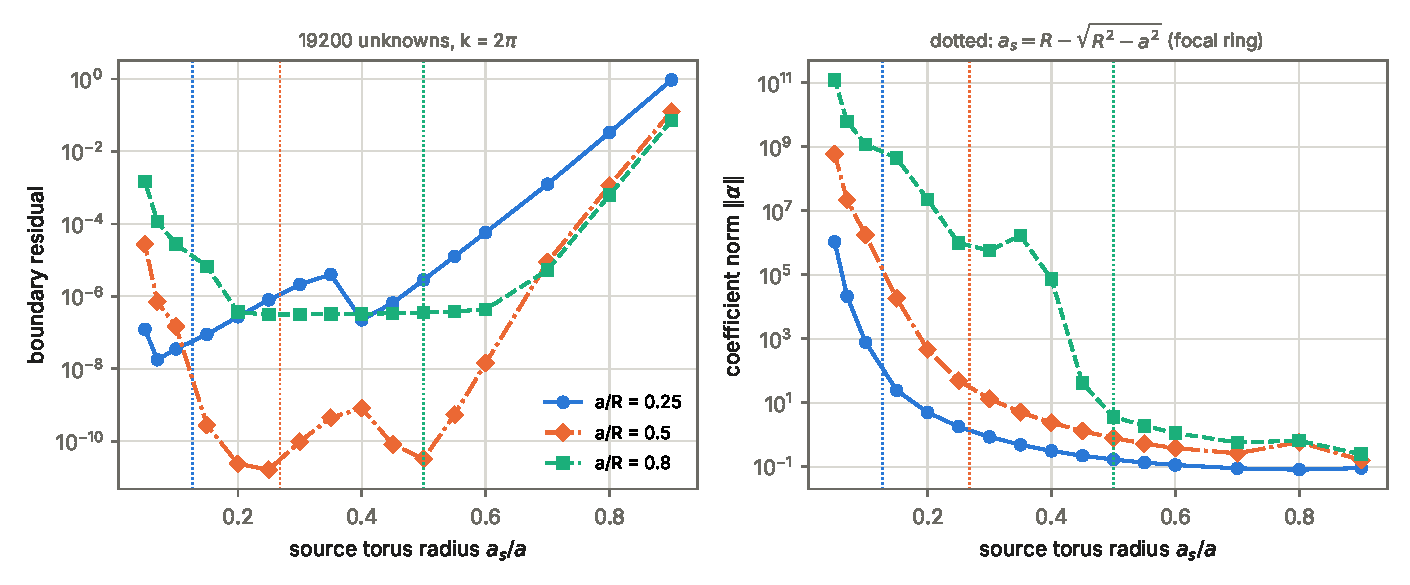
\includegraphics[width=\textwidth]{fig_torus_sources.pdf}
  \caption{Torus with $R = 1$ and three minor radii $a$, $k = 2\pi$, $19200$ unknowns. Boundary residual (left) and coefficient norm (right) against the radius of the source torus. The dotted lines mark the bound \eqref{eq:torusradius}.}
  \label{fig:torussources}
\end{figure}

\subsection{Results}

We take $a_s = 0.5\,a$, which satisfies \eqref{eq:torusradius} for $a/R = 0.5$. \autoref{tab:torus} lists the error of the scattered field against the finest MFS run, which has $40320$ unknowns, a boundary residual of $1.1\times10^{-10}$ and an optical mismatch of $9\times10^{-14}$. The error falls from $5.0\times10^{-3}$ with $1440$ unknowns to $7.3\times10^{-12}$ with $21120$ unknowns, and the finest of these runs takes $7.0$\,s. For a wave arriving obliquely, from the polar angle $60^\circ$ and the azimuth $25^\circ$, the boundary residual with $21120$ unknowns is $2.6\times10^{-10}$.

There is no exact solution to compare with. Bempp with $9600$ unknowns is $8.2\times10^{-3}$ away from the MFS field after $27$\,s. Its extinction cross-section approaches the MFS value $11.7526$ like the reciprocal of the number of unknowns, and extrapolation gives $11.7533$, a relative difference of $7\times10^{-5}$.

The MFS uses the rotational symmetry of the body and Bempp does not. To separate the two effects, \autoref{tab:torus} also lists the MFS with the full matrix. Without the symmetry the MFS needs $22$\,s for an error of $1.1\times10^{-4}$. A boundary element code for bodies of revolution would gain from the symmetry in the same way.

\begin{table}[htbp]
  \centering
  \caption{Torus, $R = 1$, $a = 0.5$, $k = 2\pi$, wave along the axis: unknowns, wall time and difference from the finest MFS run.}
  \label{tab:torus}
  \begin{tabular}{lrrl}
    \toprule
    Method & Unknowns & Time [s] & Error \\
    \midrule
    MFS, mode by mode &  1440 & 0.28 & $5.0\times10^{-3}$ \\
    MFS, mode by mode &  3840 & 1.1  & $1.1\times10^{-4}$ \\
    MFS, mode by mode &  8064 & 2.5  & $5.0\times10^{-7}$ \\
    MFS, mode by mode & 13824 & 4.5  & $2.0\times10^{-9}$ \\
    MFS, mode by mode & 21120 & 7.0  & $7.3\times10^{-12}$ \\
    \midrule
    MFS, full matrix  &  1440 & 1.5  & $5.0\times10^{-3}$ \\
    MFS, full matrix  &  3840 & 22   & $1.1\times10^{-4}$ \\
    \midrule
    Bempp &  864 & 4.9 & $1.0\times10^{-1}$ \\
    Bempp & 2400 & 5.2 & $3.3\times10^{-2}$ \\
    Bempp & 4704 & 9.5 & $1.7\times10^{-2}$ \\
    Bempp & 9600 & 27  & $8.2\times10^{-3}$ \\
    \bottomrule
  \end{tabular}
\end{table}
